\section{Results}
\label{sec:results}

\Cref{fig:overview} shows a typical night and \cref{tab:accuracy,tab:bands} summarise accuracy. \vspace{2mm} This sentence follows a vertical space command on the same line and must stay visible.

\begin{figure}[t]
  \centering
  
\includegraphics[width=0.6\linewidth]{figures/flock}
  \caption{A sleeping flock at Dunmore seen from \SI{40}{m}. Each warm blob is one animal; the large blob at the lower left is a \term{huddle} of three.}
  \label{fig:overview}
\end{figure}

\begin{figure*}[t]
  \centering
  \begin{subfigure}{0.48\linewidth}
    
\includegraphics[width=\linewidth]{figures/flock}
    \caption{Before the flight.}
  \end{subfigure}\hfill
  \begin{subfigure}{0.48\linewidth}
    
\includegraphics[width=\linewidth]{figures/flock.png}
    \caption{After the flight.}
  \end{subfigure}
  \caption{Disturbance is invisible at this scale, which is the point.}
  \label{fig:pair}
\end{figure*}

\begin{table}[t]
  \centering
  \caption{Census error by method, as a percentage of the walked ground count.}
  \label{tab:accuracy}
  \begin{tabular}{llrr}
    \toprule
    \multirow{2}{*}{Farm} & \multirow{2}{*}{Terrain} & \multicolumn{2}{c}{Error (\%)} \\
    \cmidrule(lr){3-4}
     & & Dusk count & \sys \\
    \midrule
    Dunmore & lowland fringe & 6.1 & 1.2 \\
    Sk\'ali & plateau & 8.3 & 2.0 \\
    Pe\~na Alta & terraced & 7.9 & $2.3 \pm 0.4$ \\
    \bottomrule
  \end{tabular}
\end{table}

\begin{table*}
  \caption{Disturbance score by flight height band.}\label{tab:bands}
  \centering
  \begin{tabular}{l|c|c}
    \hline
    Height band & Nights & Mean score \\
    \hline
    20--30\,m & 9 & 0.11 \\
    30--50\,m & 21 & 0.03 \\
    \hline
  \end{tabular}
\end{table*}

\begin{algorithm}[t]
\caption{Counting warm bodies in one thermal frame}\label{alg:count}
\begin{algorithmic}[1]
\Require frame $\heat$, threshold $\wake$
\Ensure count $\hat{N}$
\State $B \gets \Call{Blobs}{\heat > \wake}$
\State $\hat{N} \gets 0$
\For{each blob $b \in B$}
  \If{$\mathrm{area}(b) > a_{\max}$} \Comment{a huddle}
    \State $\hat{N} \gets \hat{N} + \Call{SplitHuddle}{b}$
  \Else
    \State $\hat{N} \gets \hat{N} + 1$
  \EndIf
\EndFor
\State \Return $\hat{N}$
\end{algorithmic}
\end{algorithm}

The reference implementation is short:
\begin{lstlisting}[language=Python, caption={Blob counting: all of the logic}]
def count(frame, tau):
    # a comment with a % sign and a $ sign, and \begin{equation}
    blobs = label(frame > tau)

    return sum(split(b) if b.area > A_MAX else 1 for b in blobs)
\end{lstlisting}

Raw flight logs look like this:
\begin{verbatim}
2031-10-04T02:11:09Z  alt=41.2m  temp=6.5C  score=0.02  % not a comment
\section{This is not a heading}
$ unbalanced { braces
\end{verbatim}

The pipeline is sketched below.

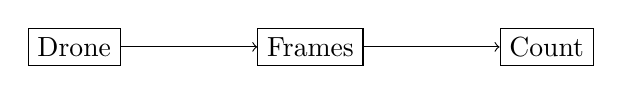
\begin{tikzpicture}
  \node[draw] (a) at (0,0) {Drone};
  \node[draw] (b) at (3,0) {Frames};
  \node[draw] (c) at (6,0) {Count};
  \draw[->] (a) -- (b);
  \draw[->] (b) -- (c);
\end{tikzpicture}

\medskip
\begin{center}
Centred text is still prose and must be shown.
\end{center}

\newpage
Results continue on a new page. Line one of an address \\ line two of an address \\[4pt] line three.
\clearpage
